\begin{figure}[bth!]
 \begin{center}
	\makebox[\textwidth][c]{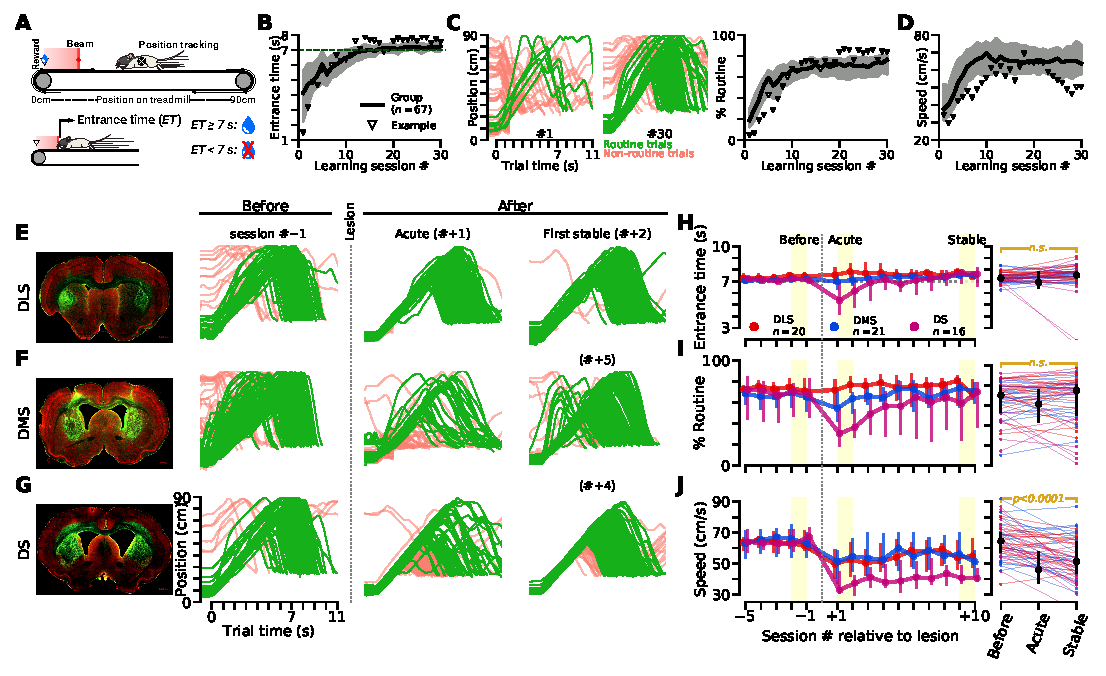
\includegraphics[scale=1]{ch-lesion/figures/Task_Example_Group.pdf}}
	\caption[The Striatum Energizes Motor Routines]
	{\textbf{The striatum is necessary to energize the running component of a motor routine.}
	\textbf{(A)} Experimental apparatus and task rules.
	\textbf{(B-D)} Performance across training sessions and animals.
	Shaded areas represent the 2nd and 3rd quartiles. Triangles represent the changes in performance of an example animal. 
	All the trajectories of this animal during sessions \#1 and \#30 are shown in C (left). 
	\textbf{(E-G)} Histology (1st column, GFAP in green shows gliosis, red is Neun) and trajectories from single animals with bilateral lesions of the dorsolateral, dorsomedial and dorsal striatum (E: DLS, F: DMS: G: DS).
	\# indicates session number relative to lesion break.
	\textbf{(H-J)} Left, Session-by-session time course of the lesion effect on ET (H), percentage of routine usage (I) and speed when animals run toward the reward area (I).
	Right, group data statistical comparison before vs after lesion (10,000 permutations).
	}
	\label{fig:lesion:task}
 \end{center}
\end{figure}